\documentclass[border=2mm]{standalone}

\usepackage{fontspec}
\usepackage{unicode-math}

\usepackage{pgfplots}
\pgfplotsset{compat=1.18}
\usetikzlibrary{arrows.meta, 
  calc, 
  positioning, 
  decorations.pathreplacing, 
  calligraphy}

\usepackage{xcolor}
\definecolor{den-1}{HTML}{111111}   % Đen #111111
\definecolor{den-2}{HTML}{222222}   % Đen #222222
\definecolor{den-3}{HTML}{333333}   % Đen #333333
\definecolor{den-4}{HTML}{444444}   % Đen #444444
\definecolor{den-5}{HTML}{555555}   % Đen #555555
\definecolor{den-6}{HTML}{666666}   % Đen #666666

% Thiết lập vị trí đặt nhãn gốc tọa độ
\tikzset{
  >=Stealth,
  originlabel/.style={
    font=\small\sf,
    anchor=north east, % Vị trí tương đối so với gốc
    yshift=-0.1ex,     % Điều chỉnh vị trí dọc một chút
    xshift=-0.1ex      % Điều chỉnh vị trí ngang một chút
  }
}

\begin{document}

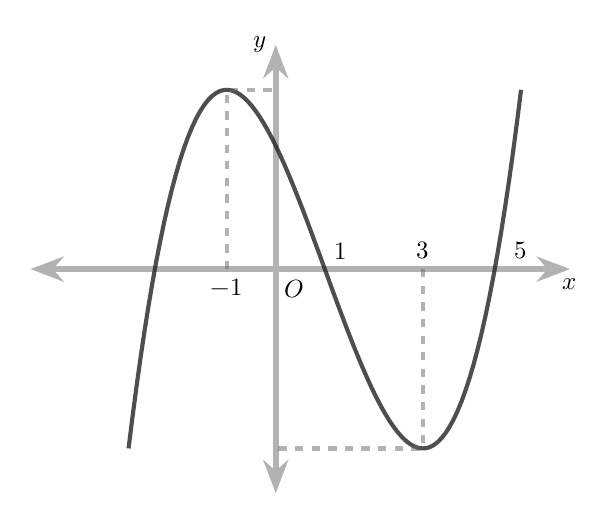
\begin{tikzpicture}
\begin{axis}[
    font=\small\sf,
    axis lines=middle,
    axis line style={<->, line width=2pt, color=den-6!50},
    xlabel=$x$, ylabel=$y$,
    xlabel style={below, font=\small\sf},
    ylabel style={left, font=\small\sf},
    xmin=-5, xmax=6,
    ymin=-20, ymax=20,
    xtick={},
    xticklabels={},
    xtick style={draw=none},
    ytick={1},    
    yticklabels={}, 
    ytick style={draw=none},
    tick label style={font=\footnotesize\sf},
    clip=false,
]

\node[originlabel] at (axis cs:0,0) [below right] {$O$};

\node at (-1,0) [below] {$-1$};

\node at (1,0) [above right] {$1$};

\node at (3,0) [above] {$3$};

\node at (5,0) [above] {$5$};

\addplot[ 
      domain=-3:5,     
      samples=100, 
      line width=1.5pt, 
      color=den-2, 
      opacity=.8
      ] 
        {x^3-3*x^2-9*x+11};

\addplot[dashed, line width=1.5pt, color=den-6, opacity=.5] coordinates {
        (-1,0)
        (-1,16)
        (0,16)
        };

\addplot[dashed, line width=1.5pt, color=den-6, opacity=.5] coordinates {
        (3,0)
        (3,-16)
        (0,-16)
        };

\end{axis}
\end{tikzpicture}

\end{document}